\documentclass[tikz]{standalone}
% \definecolor{colorrds}{HTML}{0060A0}
% \usepackage[letterpaper]{geometry}
\begin{document}
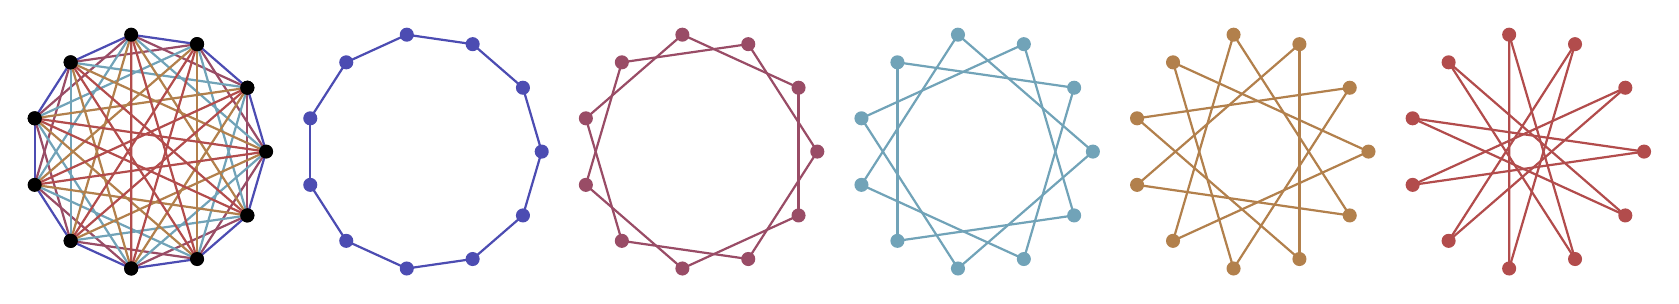
\begin{tikzpicture}
    \pgfmathsetmacro\a{360/11};
    \foreach \s/\c in {1/blue,2/purple,3/cyan,4/orange,5/red}{
            \foreach \v in {1,2,3,...,11} {
                    \draw[thick,\c!40!gray] (\v*\a:1.5) -- (\s*\a+\v*\a:1.5);
                    \begin{scope}[xshift = \s*3.5cm]
                        \draw[thick, \c!40!gray,fill=\c!40!gray] (\v*\a:1.5) circle
                        (0.075);
                        \draw[thick,\c!40!gray] (\v*\a:1.5) -- (\s*\a+\v*\a:1.5);
                    \end{scope}
                }
        }
    \foreach \v in {1,2,3,...,11} {
            \draw[thick,black,fill=black] (\v*\a:1.5) circle (0.075);
        }
    \foreach \v in {12,15,...,30} {
            \draw[thick,black,fill=black] (\v*\a:1.5) circle (0.075);
        }
\end{tikzpicture}
\end{document}